\documentclass[11pt]{article}

%────────────────────────────────────────────────
%— Your existing style
\usepackage{pepadun}

%────────────────────────────────────────────────
%— BIBLIOGRAPHY SETUP (biblatex + Biber)
\usepackage[backend=biber,style=ieee]{biblatex}
\addbibresource{pepadun.bib}
% Uncomment to include _all_ entries from pepadun.bib, even if not cited:
\nocite{*}

%────────────────────────────────────────────────
\title{Template Journal of Computing, Data, and Exploration}
\author{%
    \begin{tabular}{c}
        \textsuperscript{1}Nurlana Alili and\\
        \textsuperscript{2}Bryan Xu \\[6pt]
        \textsuperscript{1,2} Department of Mathematical and Computational Sciences, University of Toronto Mississauga, \\ 
        3359 Mississauga Road, Mississauga ON, L5M 3Z3\\[6pt]
        e-mail: \textsuperscript{1} \href{mailto:nurlana.alili@mail.utoronto.ca}{\uline{nurlana.alili@mail.utoronto.ca}}\\
        \textsuperscript{2} \href{mailto:bryansuxi.su@mail.utoronto.ca}{\uline{bryansuxi.su@mail.utoronto.ca}}
    \end{tabular}%
}
\date{}

\begin{document}

\maketitle

\begin{abstract}
In most university courses, students learn from textbooks they did not help develop. In our Independent Statistics Research Project, we as undergraduates, collaborated with faculty to create an open-access, interactive e-book for STA258: Statistics with Applied Probability – an applied statistics course at UTM that provides students their first in-depth exposure to statistical inference (hypothesis testing, confidence intervals, and related concepts).
 
In our project, we developed content, explained concepts, designed plots and figures, built interactive apps embedded in the e-book, and created illustrative examples with coding components. The e-book was created using R and Bookdown, maintained with version control (Git), and is hosted on GitHub Pages with source code available on GitHub.
 
This process made us co-authors rather than passive readers, allowing us appreciate reproducible research, collaborate, learn project management, and gain opportunities to independently learn and apply new skills. Faculty benefit from fresh ideas and perspectives.
 
In this poster, we describe the e-book’s development, methodology, software tools used, and our experience in the research process.
\end{abstract}

\section{INTRODUCTION}

In lots of undergraduate statistics classes, core concepts are introduced through traditional textbooks and lectures, which provide students with the theoretical grounding, but do not allow students an opportunity to interact with the concepts or figure out where the use of statistical methods fits in the "real world". For example, when students are learning a topic like hypothesis testing, confidence intervals, or regression, it can be very difficult for them to move from abstract theory to understanding, because of their passive learning and the lack of contextualized application of knowledge.

Recognizing these limitations, we launched an interactive e-book project in Summer 2025 as a collaboration between undergraduate students and faculty. Our desire was to totally rethink the way we deliver statistics content. We wanted to create a modern, web-based learning tool that was interactive, accessible, and engaging for students. We envisioned an interactive resource that not only explained a statistical method, but also allowed students to use live coding, dynamic visualizations, and engaged interactive applications with the statistical methods. We hoped to transform students from passive consumers of statistical methods to active participants in the use of the statistical methods, ultimately helping their comprehension and experiences with genuine learning.

Moreover, this motivation was formed from our own experiences as students trying to navigate dense lecture notes and static PDFs. We wanted to develop a resource that offered the clear, flexible, and hands-on exploration that we wished we had. In creating this vision, we wanted to adhere to the principles of reproducibility, collaboration, and open access, with the intention that our end product could be useful both to our peers and to the academic community as a whole.


\section{DESIGN, DEVELOPMENT AND IMPLEMENTATION}

The interactive e-book project was launched in the Summer of 2025 as a joint initiative between undergraduate students and faculty to create an engaging and innovative learning resource for undergraduate students enrolled in statistics courses. Our initial decision to use LaTeX was based on the appropriate typesetting features as well as its familiarity in the academic publishing landscape.

In July 2025, we decided to switch to the Bookdown framework, which we believed was better suited to the modern style of interactive and accessible online learning materials. We were able to utilize dynamic, interactive activities that greatly enhance student engagement and understanding. Converting from LaTeX (.tex) to R Markdown (.Rmd) was a seamless process using Pandoc, and most of the formatting and structure remained intact. More importantly, the Bookdown framework provided potential development features such as inline code execution, interactive graphics, and dynamic cross-referencing of equations, figures, and tables with static content being transformed into an interactive learning resource.

The effectiveness of our e-book depended on the careful selection of user-friendly, open-source tools and programming languages in order to make a visually aesthetic and reproducible learning resource. Essential technologies included:

\textbf{Languages:} R, LaTeX, Markdown, YAML, HTML5, JavaScript, CSS \\
\textbf{Packages and Frameworks:} bookdown, rmarkdown, knitr, ggplot2, plotly, Shiny \\
\textbf{Version Control and Deployment:} GitHub, GitHub Pages 

We intentionally selected these tools for inter-compatibility for working effectively together, managing version control, being transparent, and reproducible. Specifically, GitHub was primarily a repository and a node in the project for real-time collaborations on public-facing work as well as frequent updates, while GitHub Pages was a way of deploying the e-book publicly online, and also contributed to creating the conditions for others to be able to be involved asynchronously. 

Our core team consisted of two undergraduate students, Nurlana Alili and Xi Su, who both were contributors to content development and also the technical implementation; Professors Nishan Mudalige and Masoud Ataei, valuable supervisors who held regular meetings, offered substantial and specific feedback, and collaboratively shaped critical decisions regarding the e-book's structure and technology.

We received notable feedback and contributions from Dr. Steve Tully (Okanagan College) and Avanti Coonghe (United Nations, World Health Organization). Both experts provided suggestions regarding the potential scope of content, pedagogical structure, and overall educational effectiveness of the e-book development.

We faced some technical challenges, especially with the transition from LaTeX to Bookdown, but these challenges only made us more effective at comprehending reproducible computing and what collaborative digital authorship looks like. The e-book that we developed represented not only an innovative way to deliver educational content but also an adventurous journey into collaborative practices to develop and deliver meaningful academic resources.

\begin{pepadunfigure}{GitHub repository structure showing organized files, collaborative development history, and team contributions for the e-book project. GitHub supported version control, content management, and public access through GitHub Pages.}
    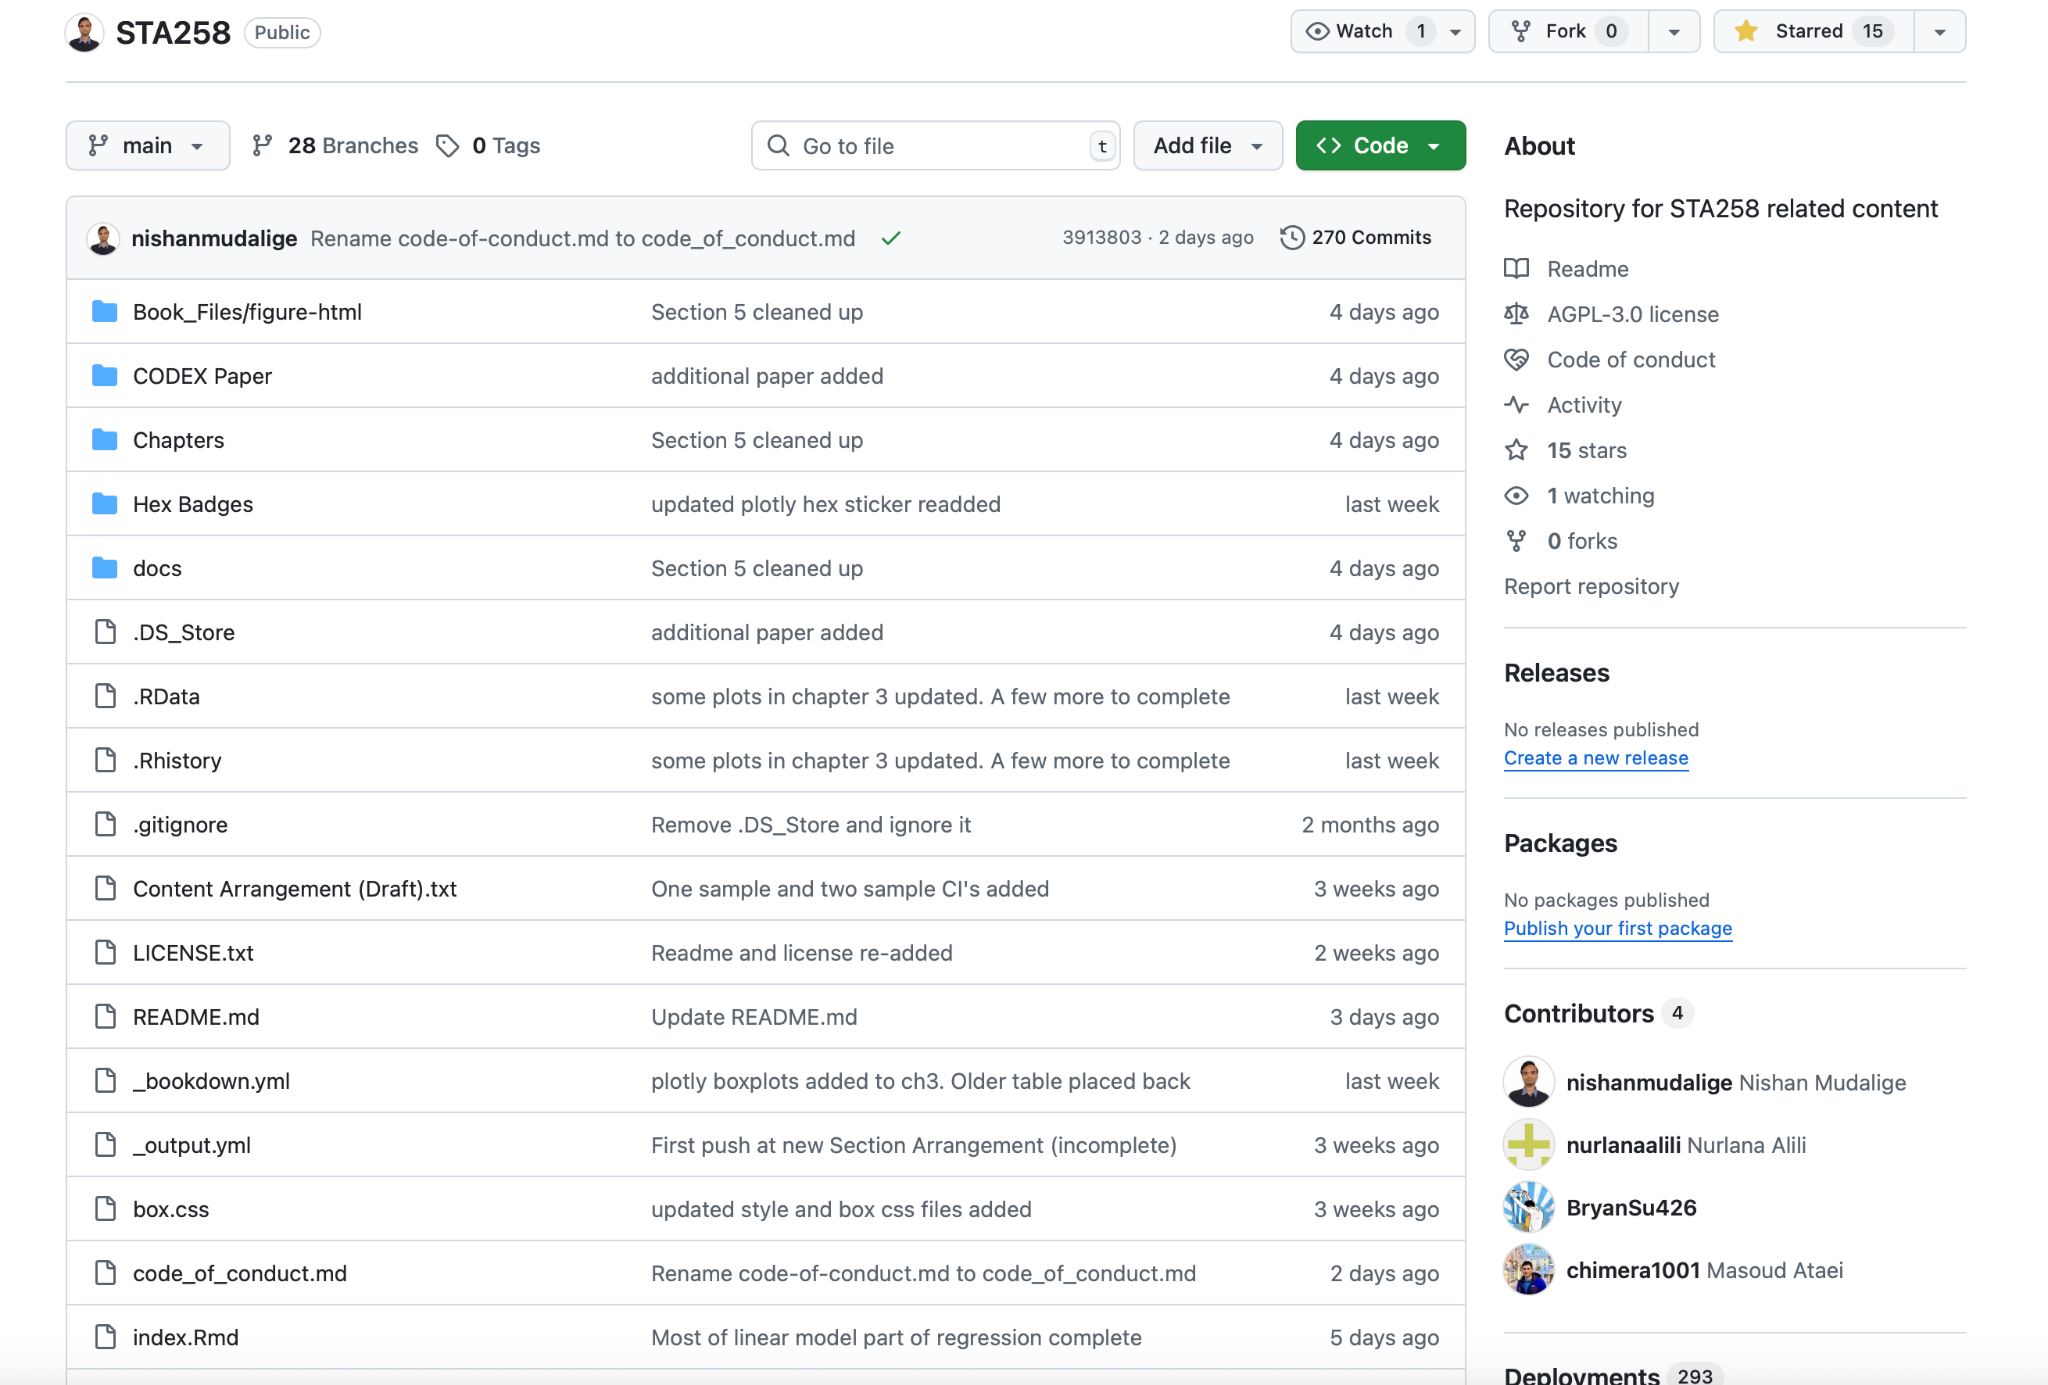
\includegraphics[width=0.7\textwidth]{Images/github-ss.png}
\end{pepadunfigure}

\section{CONTENT AND INTERACTIVE DESIGN}

Overall, this e-textbook development and formation required a considerable amount of work regarding consideration and planning to ensure that it produced a cohesive and pedagogically relevant organization. The first draft was mainly just a collection of numbered lecture notes and presentation slides; as a result, we wrote a full version using LaTeX, as this will also allow us to cohesively organize the format and style. However, when we reviewed the draft, we realized there were far too many chapters, which resulted in too much fragmentation of related content from a student's perspective. As we discussed and collaborated on the writing, we were able to put together overlapping sections and flow the material into a more logical order altogether, reducing redundancies in the end, and providing a cohesive user experience for both students and instructors.

The final outline starts with basic statistical ideas, defining important terminology, data types, and inferential statistics. We recognize the opportunities to apply statistics and have included a chapter early on R programming and when and how to apply it. This all moves quickly through a chapter that clearly explains how to install R and includes explanations of essential functions, data structures, and visualization. Therefore, we provided a solid technical foundation. Once technical skills are established, the textbook walks logically through core statistical methods, starting with the basics of inference, then to confidence intervals, hypothesis testing, and statistical power. The progression continues to more advanced material, including topics such as analysis of variance, simple linear regression, and categorical data analysis. This means students can develop their statistical reasoning in small increments, and instructors can teach from a well-defined plan of knowledge progression that will allow easy instruction.

One of the most significant challenges we encountered in creating this e-textbook was creating statistical ideas using visualizations, while ensuring the figures were educationally useful and aesthetically appealing. Initially, we relied on the TikZ package in LaTeX to create static diagrams, which were appropriate for simple illustrations. When considering more complicated statistical ideas, we understood that static figures alone were not able to demonstrate the range of dynamic ideas we needed to illustrate. For example, we found that (potentially) the simplest idea, variations in correlation between two random variables and how that affects data behaviour, was complicated to visualize. We were able to explain this theoretically and discuss the concepts behind it, but not being able to show variations in correlation in an interactive way took away from a potentially rich learning experience for the students. After facing this challenge with the static diagrams, we revisited our overall approach to visualizing statistical ideas, and we moved to R Markdown and then R Shiny to create interactive web applications in the R environment. At that point, it meant we could create dynamic visualizations with user-controlled engagement, allowing the students to manipulate variables and observe how distributions behaved. It took considerable time through trial and error to build each of these tools, including programming and redesigning to ensure the tools functioned properly, and created an exploratory learning experience.

One of the most noteworthy results—and often mentioned selling points of the e-textbook—was the collection of beautiful, publishable figures that we created in ggplot2. These images are not only aesthetically pleasing figures, with added interactive components where appropriate, but they are also far superior to traditional course materials. They reflect exact design decisions grounded in data, and they translate data into clearly stated and elegant designs that allow complex statistical concepts to be expressed intuitively and engagingly. While designed as static images and as interactive representations was labourious, it almost proved to be the most enjoyable and transformative aspect of the entire project.


\begin{pepadunfigure}{Interactive Shiny app exploring the relationship between two variables at varying correlation levels. Users can dynamically adjust the correlation coefficient and sample size, and optionally display the regression line. This tool helps students visualize how correlation strength influences the spread and direction of data points, reinforcing conceptual understanding through real-time feedback.}
    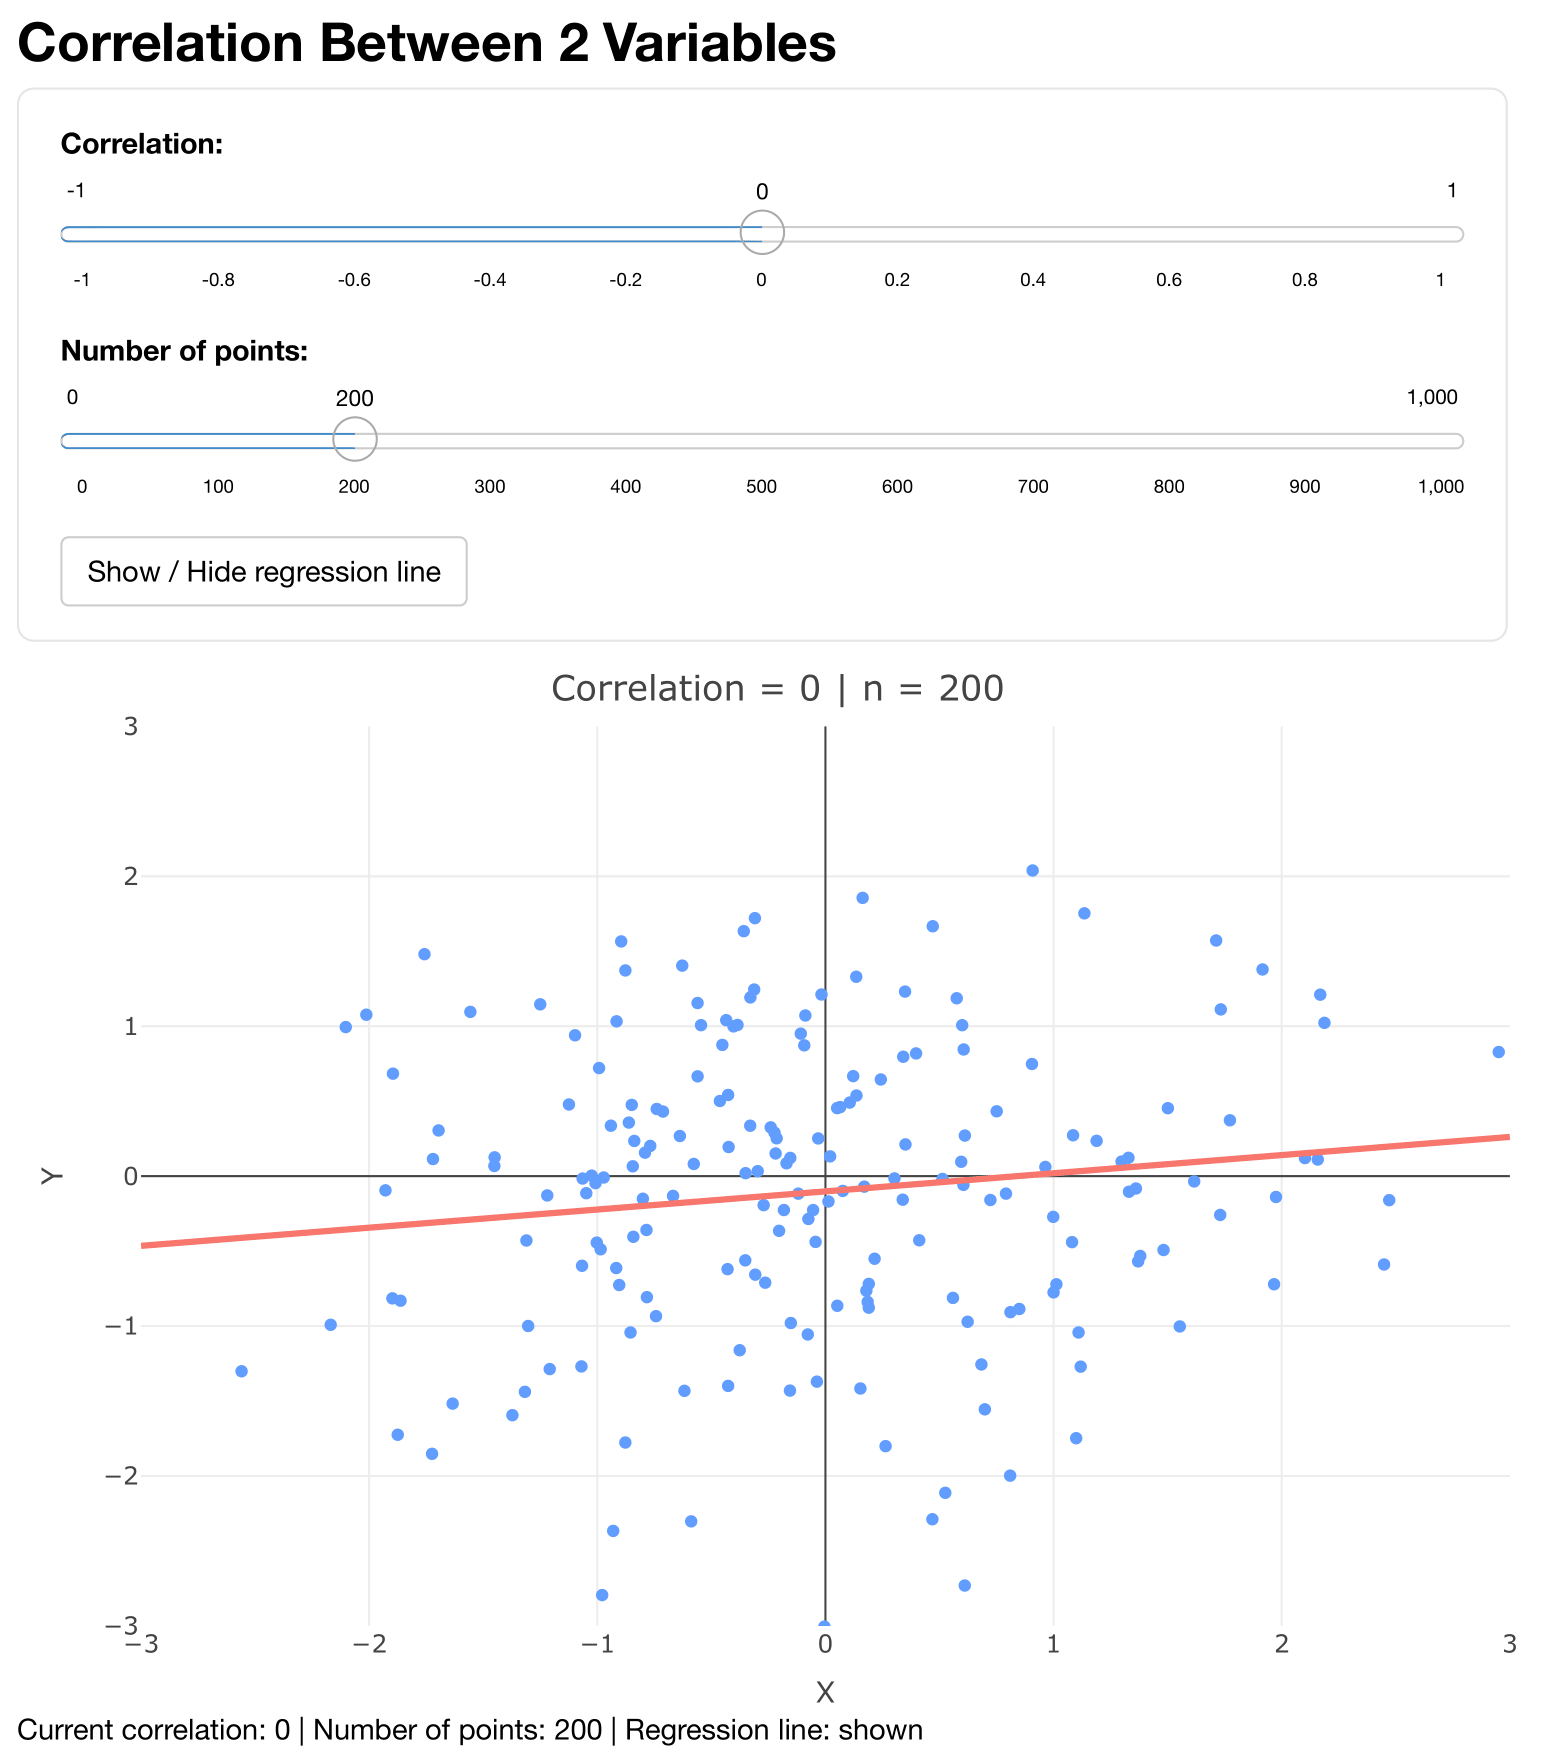
\includegraphics[width=0.7\textwidth]{Images/ch9-image.png}
\end{pepadunfigure}

\section{CONCLUSION}

In addition to technical and pedagogical impacts, our project serves as an example of the potential for student-led innovation to transform spaces of learning. It blurred the boundary between learners and educators, with students taking a role in the contribution of knowledge as opposed to being passive consumers of knowledge. This creative act required more than programming and analysis skills and additionally incorporated flexibility, purpose, and critical thinking - all increasingly useful in an academic or professional context.

From our experience, when students are given the task of authorship and design, they find a sense of investment in their learning and creative process. When students have accountability for their ideas, they take more ownership, which leads to deeper engagement with the material at hand. In the case of our project, the product or outcome was explicitly collaborative, bringing together self-reports, negotiation, and problem-solving, not limited to the domain of statistics.

Looking ahead, we are confident that this project will inspire ongoing conversation surrounding participatory curriculum design and the implications of open-source technologies as means of promoting educational innovation. It serves as a tangible opportunity for us to imagine how substantive educational change might also be realized through collaboration, interdisciplinary thinking, and creative problem-solving, which supports more inclusive and engaging learning.

\section{FUTURE WORK}

While the current iteration of the e-book is successful in embedding core statistical ideas with interactive elements, there are multiple pathways for future development. First, the central area of interest is potentially expanding the existing content to encompass more advanced topics such as generalized linear models, non-parametric tests, or multivariate analysis, so that this resource could be used with students in upper-year or specialized courses. 

Another area of focus is the enhancement of accessibility and user experience. Potential advancements include optimizing the interface for potential mobile users, incorporating text-to-speech, and offering multilingual support so that the book can reach various students from different backgrounds.

From a technical standpoint, future versions could contemplate a deeper experience with Shiny dashboards, where the reader has the opportunity to manipulate a live dataset and engage the reader in convincing, unique statistical results arranged within the proposed chapter. Ideally, embedded quizzes, automatic checking of code supplied by readers, and notes contributed by users would all contribute to a better overall experience for learners and increased retention of concepts.

In short, our long-term plan is for the project to continue to grow, particularly through ongoing student and faculty collaboration. In this way, we see a versioning system, a pipeline for documenting, and a guide for potential contributors all contributing to an established resource that future cohorts can utilize to iterate and continuously maintain as a living educational resource.


\begin{acknowledgments}
We extend our deepest gratitude to Professor Nishan Mudalige, the lead academic supervisor for this project from the beginning. His mentorship, vision, continued support, and enthusiasm were essential to the direction and actual success of this project. We are also thankful to Professor Masoud Ataei for his valuable guidance throughout the later stages of development and for his thoughtful feedback on both technical and pedagogical aspects.

We would like to thank our fellow collaborators for their contributions, and the Department of Mathematical and Computational Sciences at the University of Toronto Mississauga for creating an environment that supports vibrant student-faculty collaborations that continue to innovate.

Finally, we acknowledge the open-source community, whose many tools, documentation, and knowledge have made the technical realization of this project possible.
\end{acknowledgments}

%────────────────────────────────────────────────
%— Updated bibliography command
\printbibliography[title={REFERENCES},heading=bibintoc]

\end{document}
